\documentclass[french]{article}

\usepackage{amsmath} % for \text
\usepackage{amssymb} % for \mathbb
\usepackage{amsthm} % for proof environment
\usepackage{hyperref} % for \autoref
\usepackage{cleveref} % for \cref
\usepackage{tikz} % for tikzpicture
\usepackage{graphicx} % for \includegraphics
\usepackage{subcaption} % for subfigure
\usepackage{float} % for H in figure
\usepackage{geometry} % for \newgeometry
\usepackage{fullpage} % for fullpage
\usepackage{babel} % for french
\usepackage[T1]{fontenc} % for french

\geometry{left = 1.8cm, right = 1.8cm}

\begin{document}

\begin{center}
    \textbf{\LARGE{Ecole Normale Supérieure de Paris-Saclay}}\\
\end{center}

\vspace{1cm}

\begin{center}
    \textbf{Rapport TER}
\end{center}

\noindent\rule{\textwidth}{0.6mm}
\bigskip
\begin{center}
    \textbf{\LARGE{TER - Voiture autonomes avec apprentissage par renforcement et lidar}}
\end{center}
\bigskip
\noindent\rule{\textwidth}{0.6mm}

\begin{center}
    \today
\end{center}

\bigskip
\begin{center}
    \textsc{Miquel Hugo}
\end{center}
\begin{center}
    \textsc{Plus Basile}
\end{center}

\begin{figure}[b]
    \centering
    \begin{minipage}[h]{0.45\textwidth}
        \raggedright
        
\includegraphics[width=0.6\textwidth]{Images/Logo-ENS-Paris-Saclay.png}
    \end{minipage}
    \begin{minipage}[h]{0.45\textwidth}
        \raggedleft
        
\includegraphics[width=0.6\textwidth]{Images/Logo-Universite-Paris-Saclay.jpg}
    \end{minipage}
\end{figure}


\newpage

\tableofcontents

\newpage

\section{Introduction}

\subsection{Contexte}

Les voitures autonomes sont un sujet de recherche très actif depuis quelques années. 
En effet, elles pourraient révolutionner le monde des transports en permettant de réduire les accidents de la route, 
de diminuer la consommation d'énergie et de réduire les embouteillages. 
Cependant, il reste encore de nombreux défis à relever pour que les voitures autonomes soient utilisées à grande échelle.
En particulier, il est nécessaire de développer des algorithmes d'apprentissage par renforcement qui permettent à une 
voiture autonome d'apprendre à conduire de manière autonome.

\subsection{Objectif et travail réalisé}
L'objectif de ce TER est de développer un algorithme d'apprentissage par renforcement qui permet à une 
voiture RC au format $1/10^{\text{ème}}$ de conduire de manière autonome sur un circuit. Dans un premier temps, nous 
avons utilisé Webots pour la simulation, gym et stable baselines pour l'apprentissage par renforcement.
Dans un second temps, nous avons transféré le réseau de neurones du simulateur à la voiture réelle.
La voiture est équipée d'un lidar qui permet de mesurer la distance entre la voiture et les murs du circuit.

\vspace{0.5cm}
\noindent
Note: Presenter Webots, la voiture réelle, la voiture sur simulateur, le lidar, le circuit etc...


\subsection{L'apprentissage par renforcement}
L'apprentissage par renforcement est une méthode d'apprentissage automatique qui permet à un agent 
d'apprendre à prendre des décisions en interagissant avec un environnement. 

\begin{figure}[H]
    \centering
    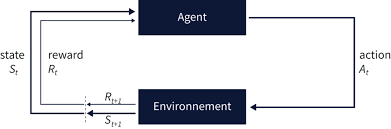
\includegraphics[width=0.6\textwidth]{Images/RL.png}
    \caption{Schéma de l'apprentissage par renforcement}
\end{figure}

\noindent
L'agent prend des actions dans l'environnement et reçoit une récompense en fonction de l'action qu'il a prise. 
L'objectif de l'agent est de maximiser la somme des récompenses qu'il reçoit au cours des itérations. 


\section{Voiture}

\section{Simulation}

\subsection{Le simulateur Webots}
\noindent
Le logiciel utilisé pour la simulation est Webots R2023b. Webots est un logiciel de simulation de robotique développé 
par Cyberbotics. Il permet de simuler des robots dans un environnement 3D que l'on peut personnaliser. Dans notre cas,
nous avons utilisé Webots pour simuler une voiture RC sur un circuit. Nous avons utilisé le langage de programmation
Python pour contrôler la voiture dans le simulateur.

\begin{figure}[H]
    \centering
    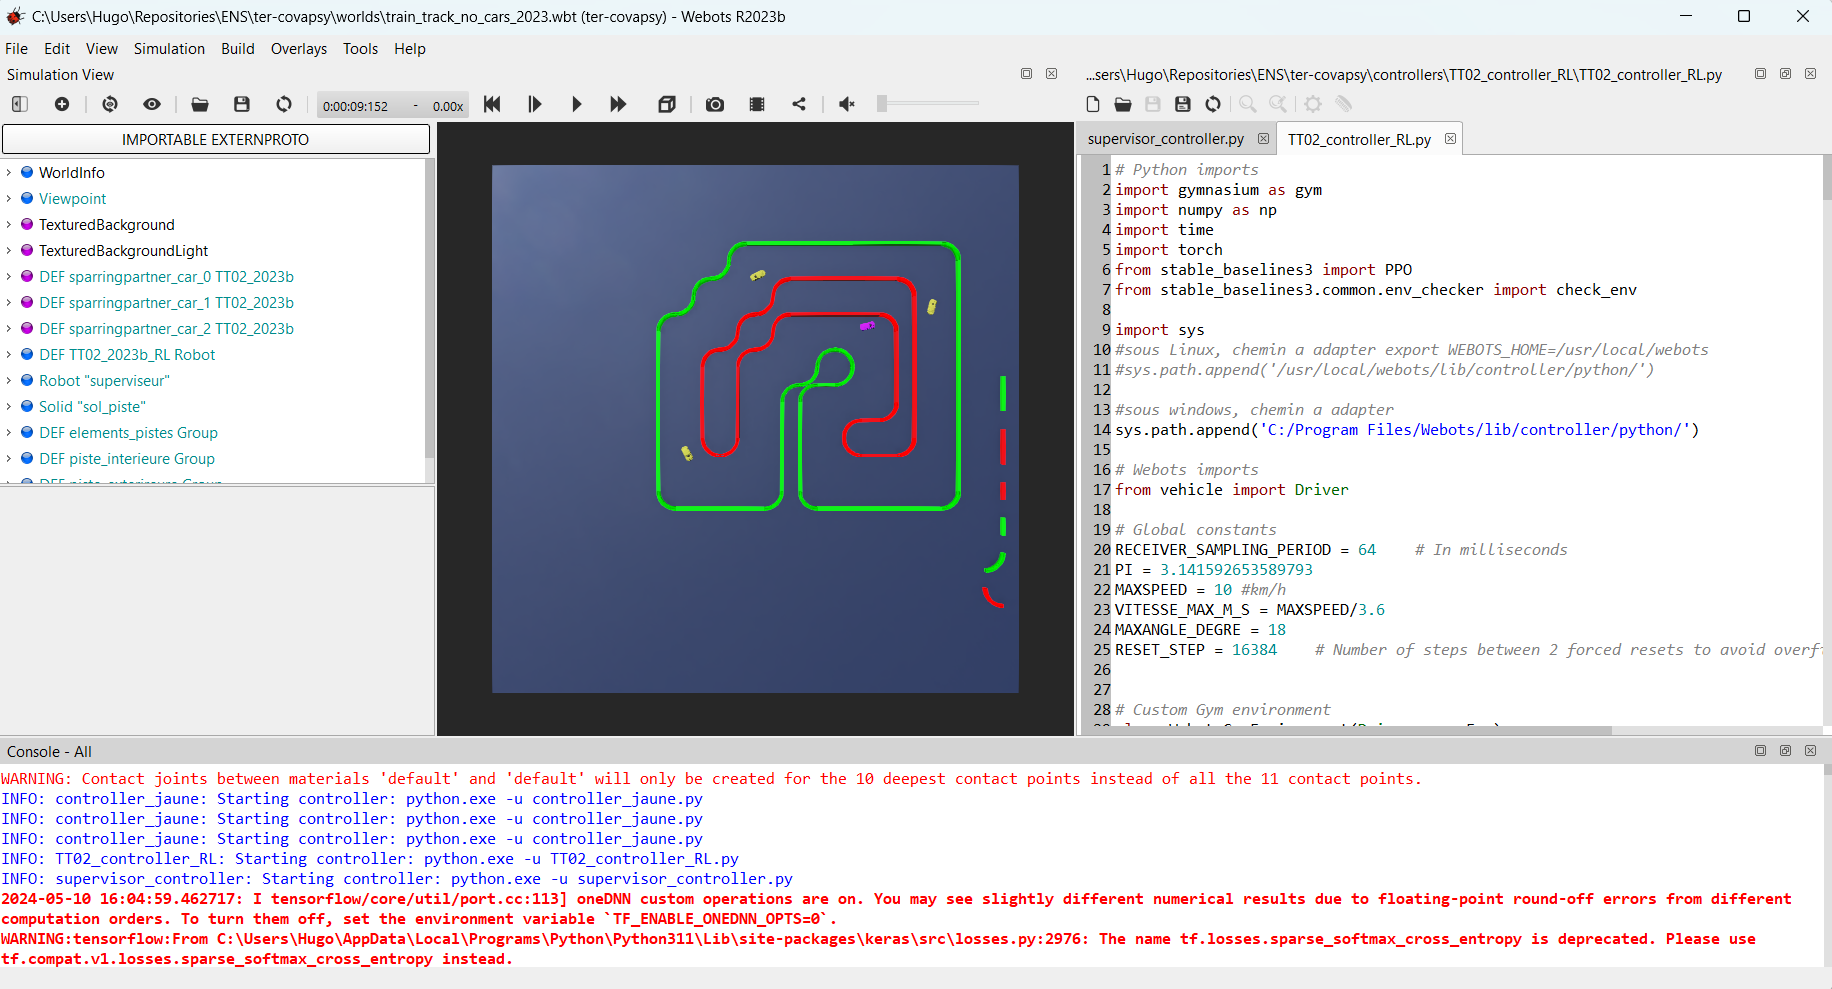
\includegraphics[width=0.9\textwidth]{Images/Webots.png}
    \caption{Capture d'écran de Webots}
\end{figure}

\noindent
Note: Présenter le circuit, la voiture, le lidar, le code Python etc...

\subsection{Le circuit}
\noindent
Le circuit dans l'environment de Webots a pour but de simuler un circuit réel sur lequel la voiture autonome doit
apprendre à conduire. Les murs du circuit sont composés de blocs de couleur différentes pour les bordures extérieur et 
intérieur du circuit. Ces murs ont une auteur d'une dizaine de centimètres qui permettent au lidar de mesurer la distance
entre la voiture et les murs.

\begin{figure}[H]
    \centering
    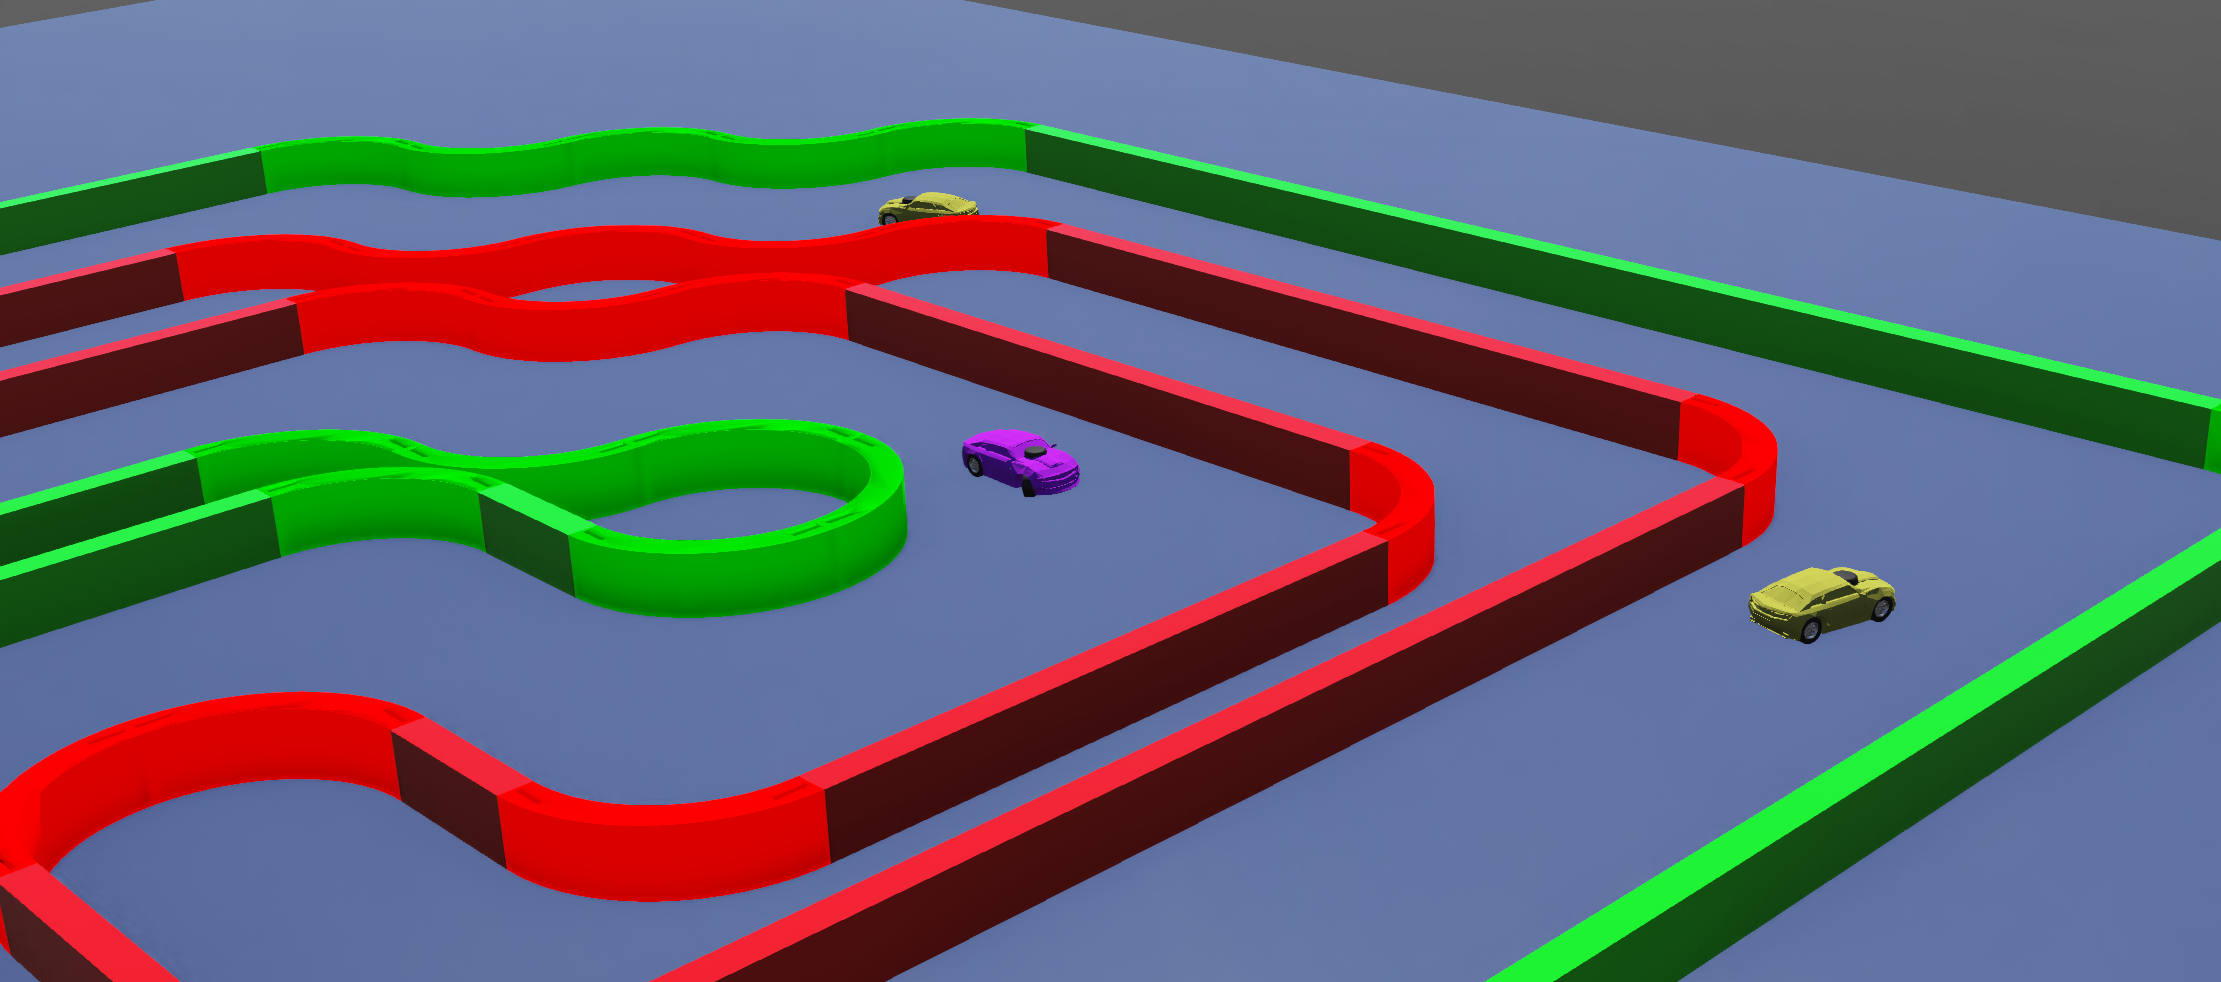
\includegraphics[width=0.9\textwidth]{Images/Circuit.png}
    \caption{Capture d'écran du circuit}
\end{figure}

\subsection{La voiture}
\noindent
La voiture utilisée dans le simulateur est une voiture RC au format $1/10^{\text{ème}}$. Elle a pour objectif de
reproduire le plus fidèlement possible une voiture réelle. La voiture est équipée d'un lidar qui permet de mesurer la
distance entre la voiture et les murs du circuit.

\begin{figure}[H]
    \centering
    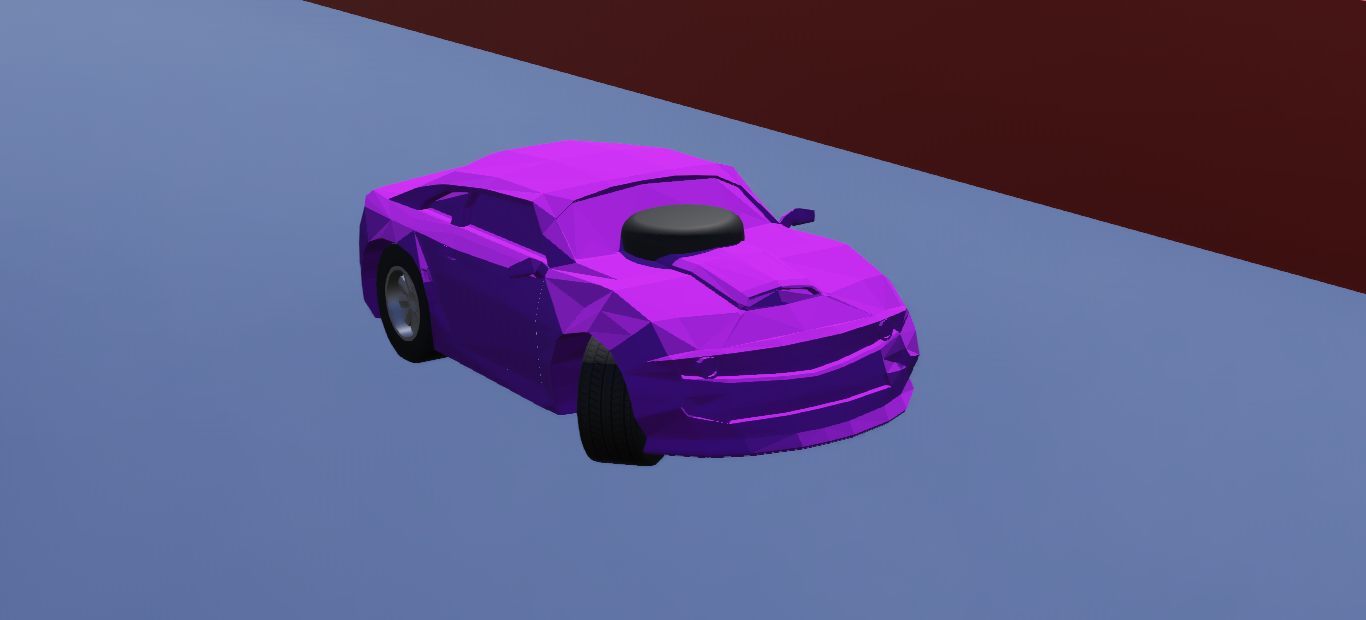
\includegraphics[width=0.9\textwidth]{Images/Voiture.png}
    \caption{Capture d'écran de la voiture}
\end{figure}

\subsection{Le lidar}


\section{Simulation to real world}
\noindent
L'objectif du SimToReal est de transférer un réseau de neurones entraîné sur un simulateur à une voiture réelle. 
Une fois le réseau de neurones entraîné, il est transféré à la voiture réelle pour qu'elle puisse conduire de manière 
autonome sur un circuit réel. Un des principaux défis du SimToReal est de reproduire le plus fidèlement possible les 
conditions du monde réel dans le simulateur.

La phase d'entraînement sur simulateur a plusieurs avantages. Tout d'abord, elle permet de réduire le temps et le coût
de l'entraînement. En effet, il est possible de simuler des milliers d'épisodes en quelques heures 
alors qu'il faudrait plusieurs jours pour réaliser le même nombre d'épisodes sur une voiture réelle. De plus,
la simulation permet de tester des scénarios dangereux pour la voiture réelle sans risquer de l'endommager.
Sur la voiture réelle, il faut aussi la replacer à la main après chaque crash dans un mur. Il est donc plus
efficace de réaliser l'entraînement sur simulateur.

\section{Introduction du bruit pour améliorer la simulation}
\noindent
Pour que la simulation soit la plus proche possible de la réalité, il est crucial d'introduire des éléments de bruit. 
Ces bruits peuvent affecter les mesures et les actions de la voiture, et ainsi permettre au réseau de neurones de 
mieux généraliser lors du passage au monde réel.


\subsection{Bruit sur les mesures}
\noindent
// a modifier nous somme en interrieur il n'uy a pas de vent etc.. mais juste un peut de bruit de mesure
Dans un environnement réel, les capteurs ne fournissent pas des mesures parfaites. Par exemple, les mesures 
du Lidar peuvent être affectées par des interférences, des réflexions multiples ou des conditions météorologiques. 
Pour simuler ces conditions, on peut ajouter du bruit gaussien aux mesures du Lidar. Cela permet au réseau de neurones 
de s'adapter à des données moins parfaites, similaires à celles qu'il rencontrera dans le monde réel.

\subsection{Bruit sur les actions}
\noindent
Les actions de la voiture, telles que l'angle de direction ou la vitesse, peuvent également être sujettes à des 
variations imprévues. Par exemple, un servomoteur peut ne pas toujours répondre de manière identique à une même 
commande en raison de l'usure ou des variations de tension. Pour prendre en compte ces imperfections, on peut 
ajouter du bruit aux actions commandées par le réseau de neurones. Cela aide à rendre l'agent plus robuste face 
aux variations qu'il pourrait rencontrer sur une voiture réelle.




\section{Application à la voiture autonome}
\noindent
Pour appliquer l'apprentissage par renforcement à une voiture autonome, il est essentiel de définir correctement 
l'espace d'observation et l'espace d'action en tenant compte des contraintes du monde réel.

\subsection{Espace d'observation}
\noindent
L'espace d'observation doit inclure toutes les informations pertinentes que la voiture peut obtenir de son environnement.
Dans notre cas, nous utilisons le Lidar pour mesurer les distances aux obstacles. Si un système de contrôle de 
la vitesse est en place, la vitesse actuelle de la voiture pourrait également faire partie de l'espace d'observation.

\subsection{Espace d'action}
\noindent
L'espace d'action est limité aux commandes que l'agent peut envoyer à la voiture. Cela inclut l'incrémentation de 
l'angle de direction via le servomoteur et l'incrémentation de la vitesse via le moteur.



\section{Conclusion}


\end{document}